\newpage
\section{Product Requirements}

\subsection{Hardware}
The custom built hardware contains all necessary components integrated on a single \acrfull{pcb}. The hardware needs to comply with the following requirements: 
\begin{itemize}
		\item The hardware shall be based around an \gls{stm32} microcontroller.
		\item The hardware shall be able to do altitude measurements for independent operation.
		\item The hardware should use a wireless communication method to receive commands.
		\item The hardware should be able to do detect if the parachute was ejected (e.g. light sensor).
		\item The hardware shall be battery operated.
		\subitem The battery shall last at least 6 hours.
		\subitem A battery management system should be added to charge and monitor the battery.
		\item The hardware shall be enclosed in order to minimize dust and moisture getting into the system.
		\item The hardware shall weigh less than 150g
		\item The hardware shall have dimensions no bigger than 80x50x30mm
		\item The hardware shall be able to indicate the current device status (e.g. \acrshort{led}, buzzer).
		\item The hardware should have an \acrshort{usb} interface for configuration.
\end{itemize}
\medskip
\begin{figure}[h!]
	\centering
	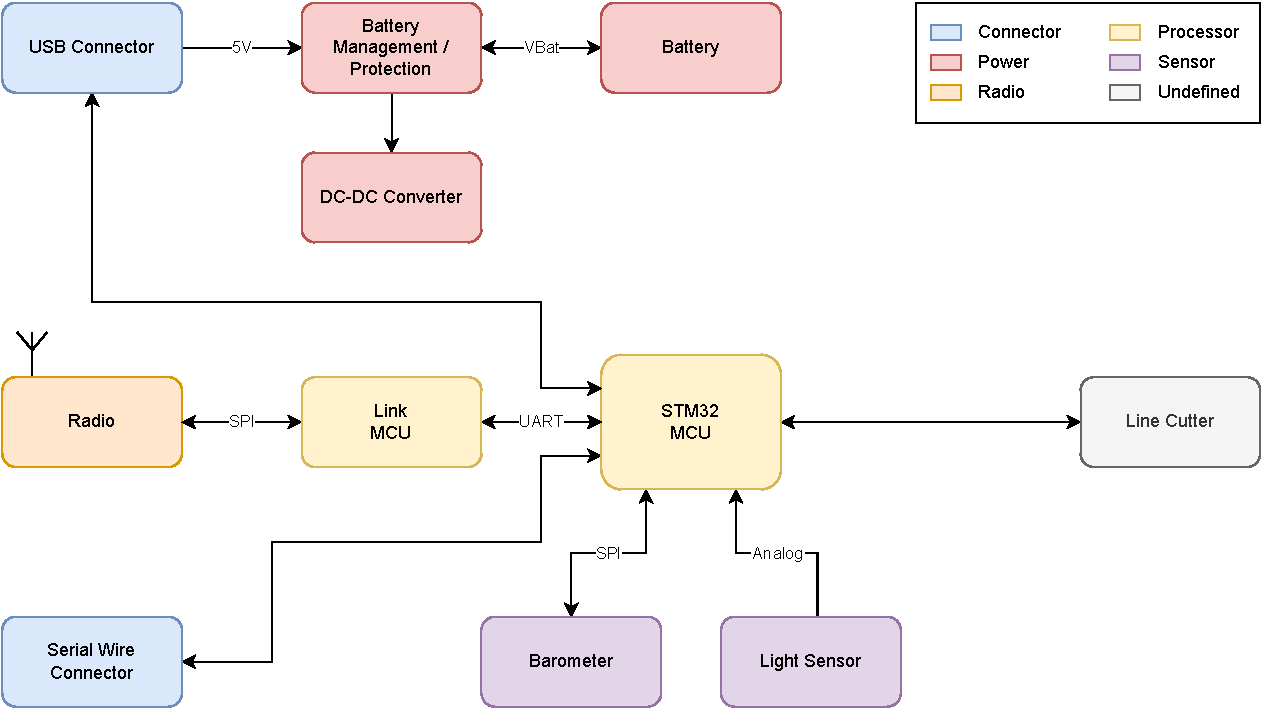
\includegraphics[height=7.3cm]{images/block_diagram}
	\caption{Example Hardware Block Diagram}
	%\vspace{-2ex}
	\label{fig:hardware_block_diagram}
\end{figure}

\newpage

\subsection{Line cutting mechanism}
The line cutting mechanism will be specifically developed for this application and needs to follow these requirements: 
\begin{itemize}
		\item The mechanism shall be able to separate the line in less than 10 seconds.
		\item The mechanism shall be reliable.
		\item The mechanism shall withstand forces acted on it during the deployment of the parachute

\end{itemize}


\label{sec:firmware}
\subsection{Firmware}
The embedded firmware will run on a \gls{stm32} and will be written in C. The requirements for the firmware are as follows:
\begin{itemize}
    \item The firmware shall connect to the transmitter.
    \item The firmware shall initiate the separation when commanded to.
    \item The firmware shall read air pressure data.
    \item The firmware shall be able to initiate the separation at a set altitude without a telemetry link.
    \item The firmware shall display the current device status to the user.
    \item The firmware shall offer an interface to configure the device through \acrshort{usb}.
\end{itemize}
